\documentclass[11pt, oneside]{article} 
\usepackage{geometry}
\geometry{letterpaper} 
\usepackage{graphicx}
	
\usepackage{amssymb}
\usepackage{amsmath}
\usepackage{parskip}
\usepackage{color}
\usepackage{hyperref}

\graphicspath{{/Users/telliott/Github/precalculus/fig/}}
% \begin{center} \includegraphics [scale=0.4] {gauss3.png} \end{center}

\title{Value of pi and Gregory}
\date{}

\begin{document}
\maketitle
\Large
\label{sec:Gregory}

As discussed in a previous \hyperref[sec:Value_of_pi]{\textbf{chapter}}, Archimedes used paired inscribed and circumscribed polygons to develop an iterative procedure that can be used to calculate the value of $\pi$ \emph{to any desired accuracy}.  

Although the method is beautiful, his argument is unwieldy in detail, so we used modern trigonometry to achieve the same result more economically.

There are, in addition, two other sets of formulas that also reach this end, one based on perimeters, and the other on areas.  These formulas are intriguing because they are simple, and it is not surprising that they are connected.  

For example, consider a circle of unit \emph{diameter}, so that $\pi$ is equal to the perimeter.  If $p$ and $P$ are the inside and outside perimeters for polygons whose sectors have central angle $\theta$, and the same symbols are used with primes for angle $\theta/2$, then:

\[ P' = 2 \frac{pP}{p + P} \]
\[ p' = \sqrt{pP'} \]

The corresponding formulas for inside ($a$) and outside ($A$) areas are (for a circle of unit radius)
\[ A' = 2 \frac{a'A}{a' + A} \]
\[ a' = \sqrt{aA} \]

Notice that these two similar sets of formulas are subtly different.  For example, to go from $p$ and $P$ to the primed version, we start with the first formula, while for area we must start with the square root.  Part of our purpose in this chapter is to show that this works.

\subsection*{inspiration}

It's striking that the formulas for the inside and outside perimeters are so simple, namely $n \sin \theta$ and $n \tan \theta$.  The rest just follows from the half-angle formulas.

The web page which originally got me started with the harmonic and geometric mean formulas has been preserved by the wayback machine:

\url{https://web.archive.org/web/20171024182015/http://personal.bgsu.edu/~carother/pi/Pi3d.html}

On the very same day that I was revising the previous chapter to better integrate these two approaches, I came across another page which gives a "proof without words" of Gregory's Theorem (that is our subject).

\url{https://divisbyzero.com/2018/09/28/proof-without-word-gregorys-theorem/}

It gives these two formulas:
\[ I_{2n} = \sqrt{I_n C_n} \]
\[ C_{2n} = \frac{2}{1/I_{2n} + 1/C_n} \]

I found this notation a bit awkward, so I substituted the versions given above:
\[ a' = \sqrt{aA} \]
\[ A' = 2 \frac{a'A}{a' + A} \]

Here, we mainly follow the development from that page and its "proof without words".  

One difference is that we will start with the geometry and work backward to the formulas.  Another is that we will use quite a few words.  Let's deal with the perimeter first and then do the area.
\subsection*{chord of a circle}
Before we start the main part, let's just establish some facts about a chord of a circle.  
\begin{center} 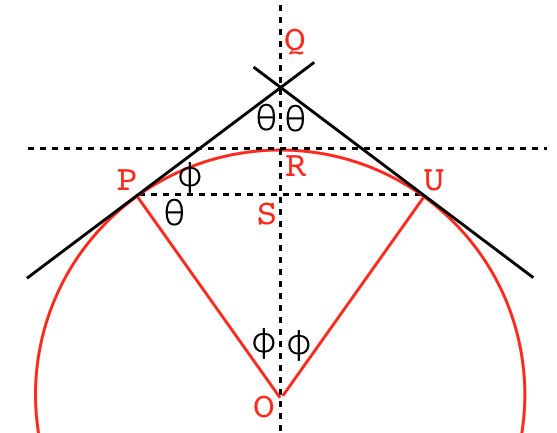
\includegraphics [scale=0.4] {Gregory_r00.png} \end{center}

Draw three radii of the circle such that the third bisects the first two, with angles equal to $\phi$ at the center, point $O$.

We will show that the chord is parallel to the tangent at $R$, and perpendicular to $OSQ$.

First, tangents are always perpendicular to the radius at the point where they meet the circle.

$\triangle OPS \cong \triangle OSU$ by SAS.  Therefore, all four angles at $S$ are right angles.  Therefore the chord $PU$ is perpendicular to $OSRQ$.  Therefore the chord is parallel to the tangent at $R$.

The other angle labels are justified as complementary angles in a right triangle.  

So any chord which is bisected in this way, is parallel to the tangent above it.  And the bisection of the chord follows from the bisection of the base angle at $O$.

\subsection*{basic setup}
\begin{center} 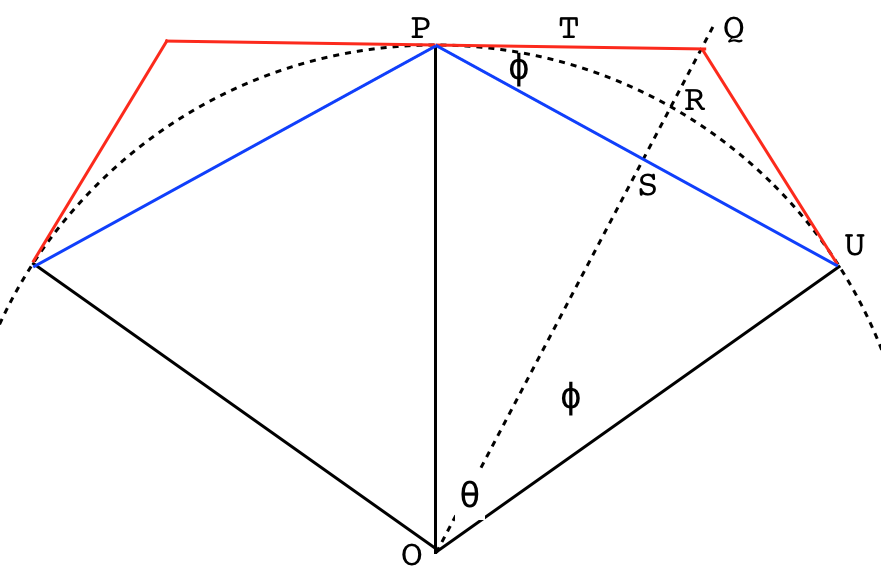
\includegraphics [scale=0.3] {Gregory_r0.png} \end{center}
Draw a circle centered at $O$ (only an part of the circle  is shown).  

Divide the whole $2 \pi$ radians into $2n$ parts such that $\phi$ is equal to one of these parts and $\theta$ is equal to two of them.  

Draw $OP$, $OR$ and $OU$ as radii, and extend $OR$ to $OQ$.

Draw the sides of a regular polygon with $n$ sides inscribing the circle and touching its perimeter at $P$ and $U$.  Similarly draw the sides of an $n$-gon circumscribing the circle and touching its perimeter at the same points $P$ and $U$.

Two red lines comprise this sector's external perimeter $P$, while a single blue line is the inscribed perimeter $p$.  The lines of the external perimeter are both tangent to the circle at $P$ and $U$, and the whole figure is symmetric in each sector, with one blue and two red lines.
\begin{center} 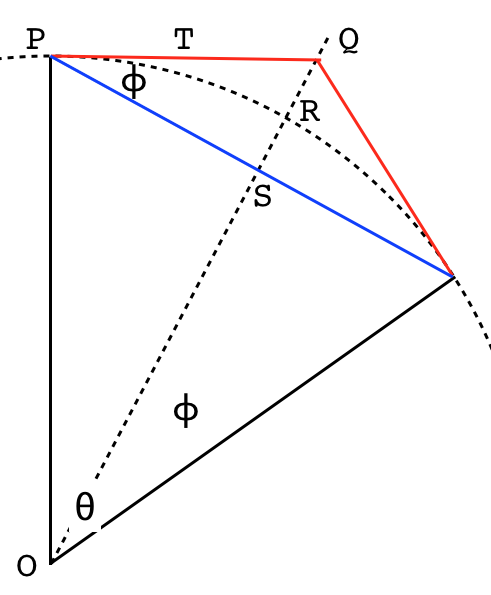
\includegraphics [scale=0.3] {Gregory_r1.png} \end{center}

By our preliminary results, $\angle PSR$ is a right angle and $\angle SPQ$ is equal to $\phi$.

And as we said, the perpendicular bisector to a chord is perpendicular to the tangent at the point where the chord intersects the circle ($R$).

\subsection*{bisecting $\phi$}

Next, draw the perimeters $p'$ and $P'$ for the polygon with $2n$ sides and sector angle $\phi = \theta/2$.

It is convenient to rotate the internal perimeter by $\theta/2$ with respect to the external one, a bit to the left when we draw $p'$ and a bit to the right for $P'$.  Both $p'$ and $P'$ touch the circle at $R$.

A central relationship we use below is that $\triangle PRT$ is isosceles.
\begin{center} 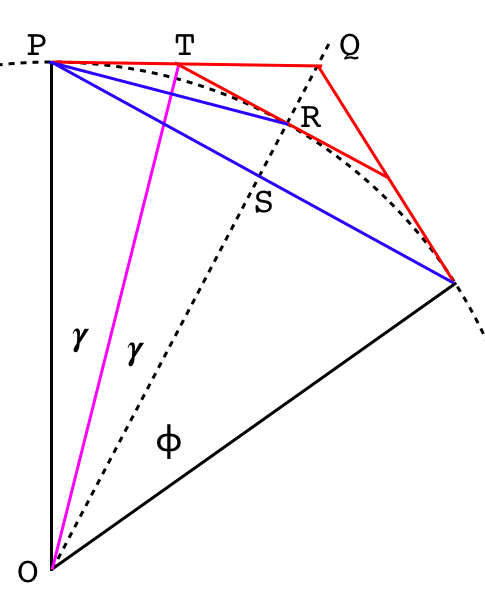
\includegraphics [scale=0.3] {Gregory_r2b.png} \end{center}

Proof.

$angle VPT \cong \angle VRT$ and the angles at $V$ are right angles, by the preliminary result.  Therefore $\angle TPV = \angle TRV$ so $\triangle PRT$ is isosceles.  By complementary angles, the base angle has measure $\gamma$.

$\square$

It looks as if the segment of the vertical that extends beyond the radius might be equal to that part below down to what looks like the "strut" of a kite.  However, this is not true.  We will show what this ratio is equal to in just a bit.

Rather than use the vertices as points of reference, let us now label the line segments.
\begin{center} 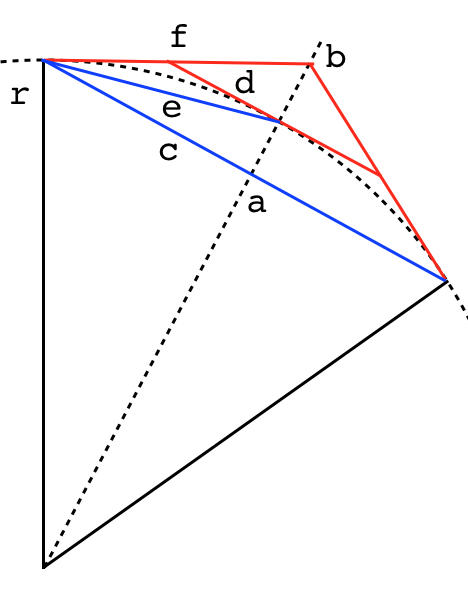
\includegraphics [scale=0.3] {Gregory_r3.png} \end{center}

Just to be clear:  $a$ is the part of the radius extended to point $S$ in the previous drawing, the intersection of the dashed black and solid blue lines, while $b$ extends all the way to $Q$, at the vertex of the circumscribing polygon.  

$c$ and $d$ are the lengths of the indicated lines \emph{in the half-sector}, not all the way across, and $f$ is the entire length of $PQ$.

We're ready to proceed.

\subsection*{perimeters}
As we said, the key observation is that $\triangle PRT$ is isosceles.  
\begin{center} 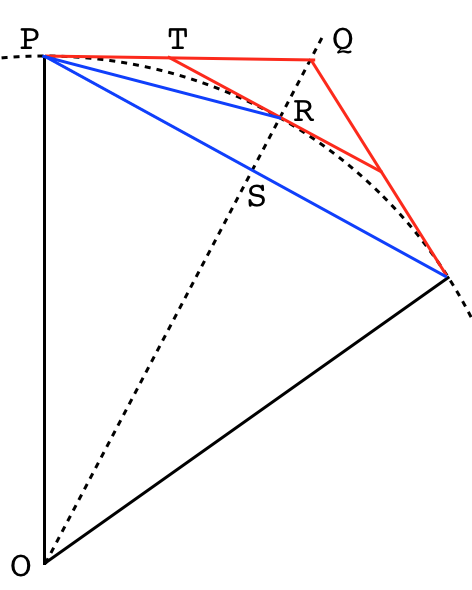
\includegraphics [scale=0.3] {Gregory_r2.png} \end{center}

Because of that, and since $\angle SPR = \angle PRT$ by the alternate interior angles theorem, $\angle SPR = \angle TPR$.  

Therefore the cosines are also equal, namely:
\[ \frac{c}{e} = \frac{e/2}{d} \]
\begin{center} 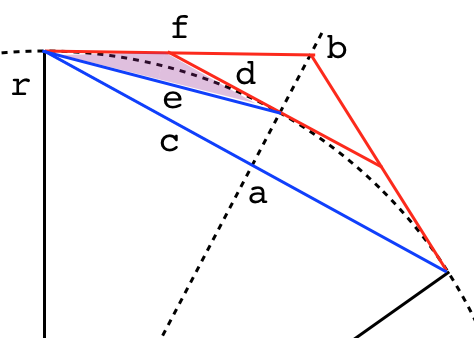
\includegraphics [scale=0.3] {Gregory_r4.png} \end{center}
(To see the midpoint of $e$, drop an altitude in the isosceles triangle, shown in purple).

Therefore:
\[ 2dc = e^2 \]
Now, $c$ is the entirety of $p$ in this half-sector.  But $d$ is only one-half of $P'$.  

Hence $2d \cdot c$ is equal to $pP'$, and since $e = p'$, we have that 
\[ pP' = [p']^2 \]
which was our second rule for the perimeters.

The first rule was
\[ P' = 2 \frac{pP}{p + P} \]

In geometric terms, we must show that
\[ 2d = 2 \frac{cf}{c + f} \]
\[ cd + df = cf \]

Taking another look at the diagram:
\begin{center} 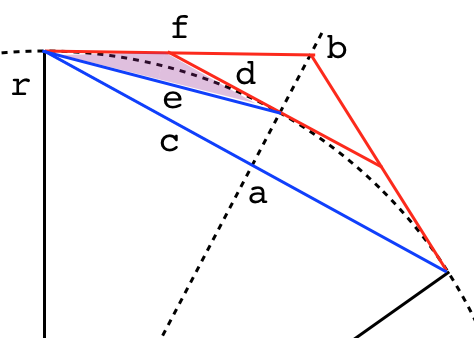
\includegraphics [scale=0.3] {Gregory_r4.png} \end{center}

The small triangle with base $d$ ($\triangle QRT$ above) has slanted side $f - d$ (subtracting $d$ because, again, $\triangle PRT$ is isosceles).  By similar triangles, we have
\[ \frac{d}{f-d} = \frac{c}{f} \]
\[ df = cf - cd \]
\[ cd + df = cf \]
Which is what we needed to prove.

$\square$

\subsection*{areas}

The area formulas for inside ($a$) and outside ($A$) polygons are those for a circle of unit radius (so that $\pi$ is the area):
\[ A' = 2 \frac{a'A}{a' + A} \]
\[ a' = \sqrt{aA} \]

This is what we will prove.

However, having reached this point, we need another symbol for area, because $a$ is currently the line segment corresponding to $p/n$.  Let's use $I$ and $C$ for the inside and outside areas, to match the source.  

We will also adopt their $n$ and $2n$ notation, It's a bit clumsy but that will make it easier to match things up.  Substituting in the above equations:
\[ C_{2n} = 2 \cdot \frac{I_{2n} C_n}{I_{2n} + C_{n}} \]
\[ I_{2n} = \sqrt{I_n C_n} \]

The first two areas are $I_n$ and $I_{2n}$
\begin{center} 
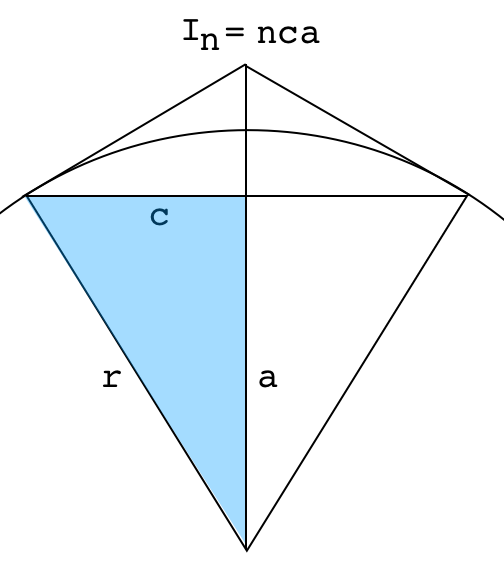
\includegraphics [scale=0.3] {Gregory1.png} 
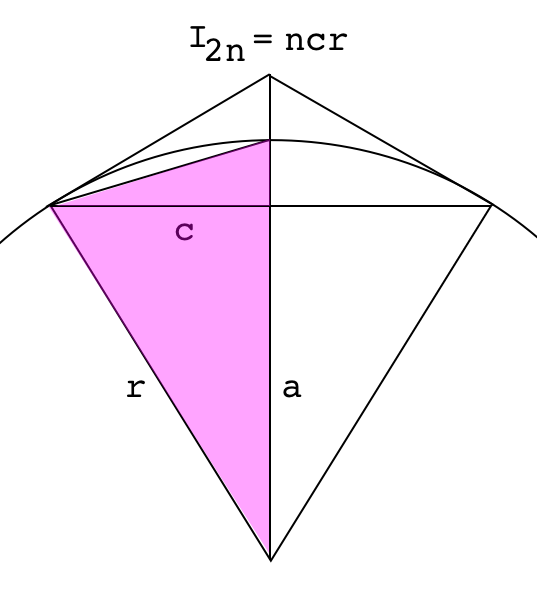
\includegraphics [scale=0.3] {Gregory2.png} 
\end{center}
We compute these areas for the whole sector of angle $\theta$, so there are two congruent triangles with base $a$ (or base $r$) and height $c$, which makes the factors of one-half go away. 

Multiply by $n$ if you like to get the entire polygon, but every expression will have a factor of $n$, and we'll be looking at ratios, so we can just not worry about it.

The third easy one is $C_n$:
\begin{center}
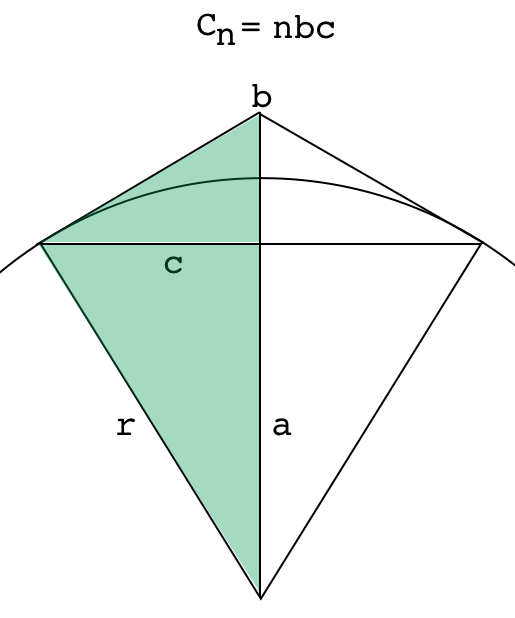
\includegraphics [scale=0.3] {Gregory3.png}
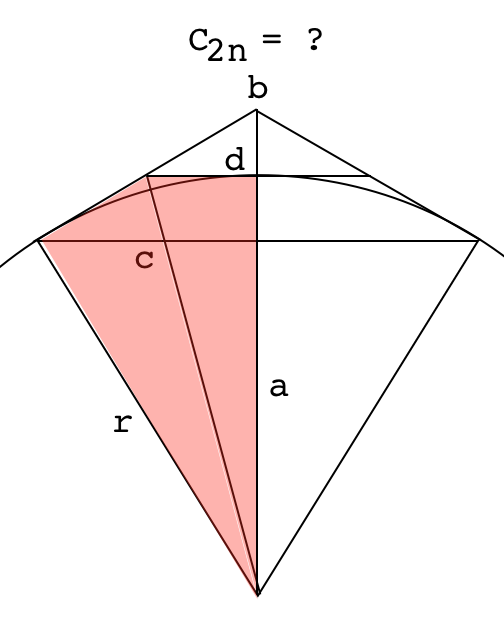
\includegraphics [scale=0.3] {Gregory4.png} 
 \end{center}
 
We write the last one ($C_{2n}$) as two different differences.
\begin{center} 
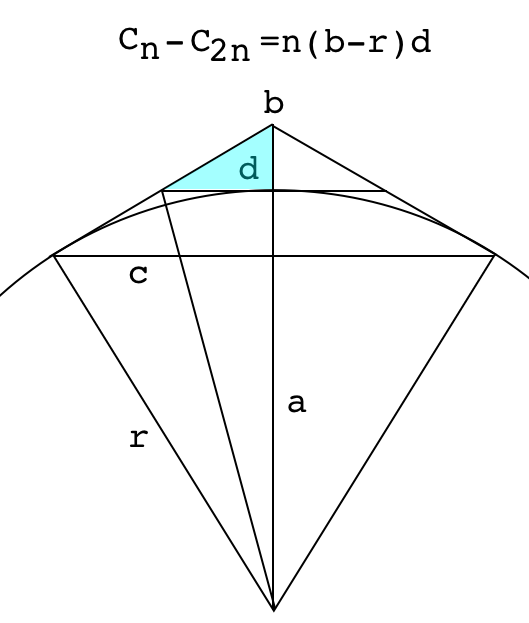
\includegraphics [scale=0.3] {Gregory5.png} 
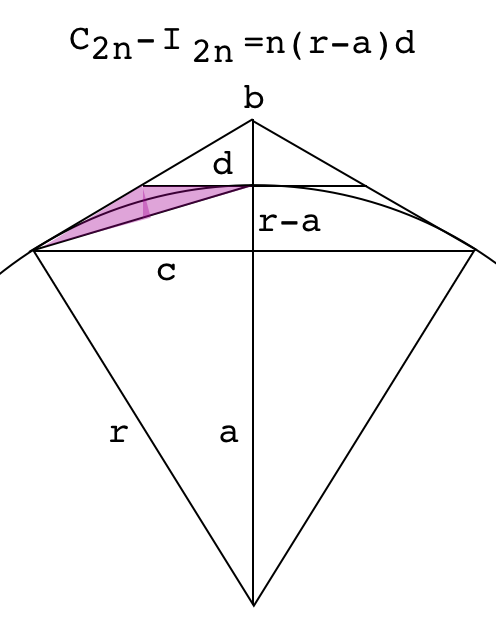
\includegraphics [scale=0.3] {Gregory6.png} 
\end{center}

Let's gather all these expressions in one place, forming ratios:
\[ \frac{I_{2n}}{I_n} = \frac{ncr}{nca} = \frac{r}{a} \]
\[ \frac{C_n}{I_{2n}} = \frac{ncb}{ncr} = \frac{b}{r}  \]
\[ \frac{C_n - C_{2n}}{C_{2n} - I_{2n}} = \frac{n(b-r)d}{n(r-a)d} = \frac{b-r}{r-a} \]

We will prove that these three ratios are all equal to each other.  

We have used the geometry to prove what the source calls their Lemmas, and those can be used in turn to prove the original Gregory formulas.

But the proof is easy:
\begin{center} 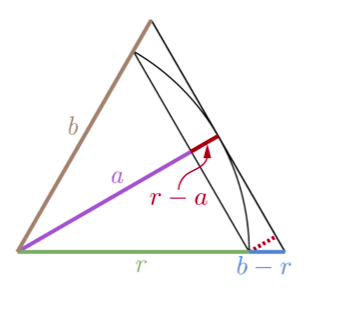
\includegraphics [scale=0.5] {Gregory7.png} \end{center}

It's just a matter of similar triangles:
\[ \frac{r}{a} = \frac{b}{r} = \frac{b-r}{r-a} \]

That's the "without words" part.

For that very last part, you can work out the dimensions of the tiny similar triangle, or you can say:
\[ \frac{r}{a} = \frac{b}{r} \]
\[ \frac{r}{a} - \frac{a}{a} = \frac{b}{r}- \frac{r}{r} \]
\[ \frac{r-a}{a} = \frac{b-r}{r} \]
which is easily rearranged to give the desired result.

$\square$

This can also be proved using the \hyperref[sec:angle_bisector]{\textbf{angle bisector theorem}}.
\begin{center} 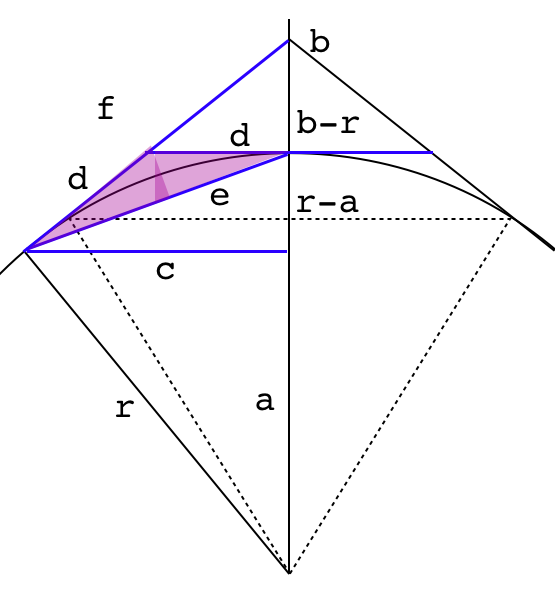
\includegraphics [scale=0.25] {Gregory10.png} \end{center}
The side labeled $e$ bisects the angle formed by the two sides labeled $c$ and $f$.  Therefore 
\[ \frac{b-r}{f} = \frac{r-a}{c} \ \ \Rightarrow \ \  \frac{b-r}{r-a} = \frac{f}{c} \]
But $f$ and $c$ are two sides of a triangle which is similar to the colored portions below:

\begin{center} 
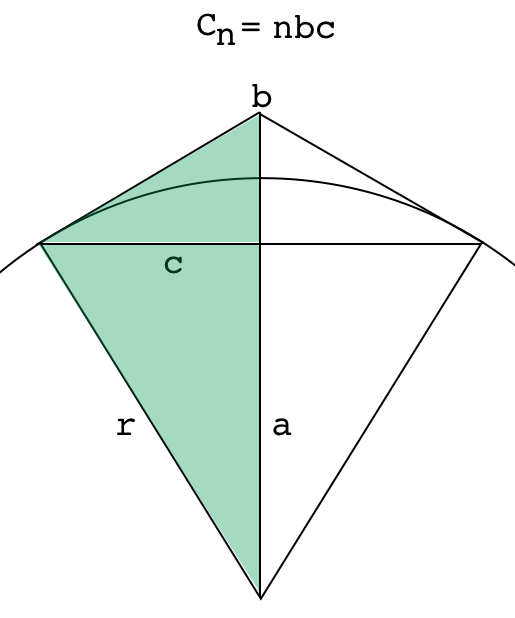
\includegraphics [scale=0.25] {Gregory3.png} 
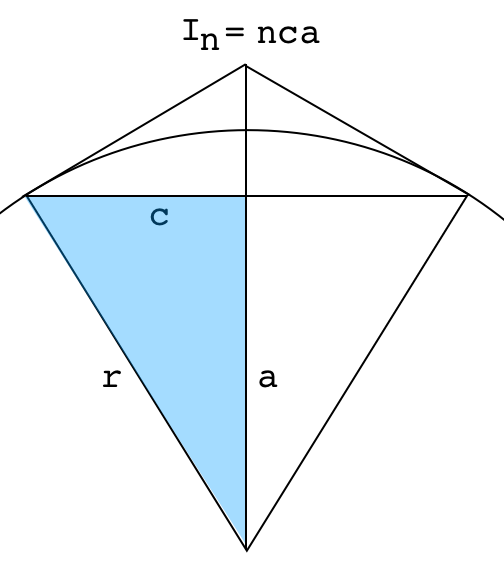
\includegraphics [scale=0.25] {Gregory1.png} 
\end{center}
Therefore
\[ \frac{b}{r} = \frac{r}{a} = \frac{f}{c} = \frac{b-r}{r-a}  \]
As we said.

\subsection*{algebra}
Moving on to the geometric mean formula is not hard.  From above we have that
\[ \frac{I_{2n}}{I_n} = \frac{C_n}{I_{2n}}   \]
\[ [I_{2n}]^2 = I_n C_n  \]
Translated back into the $A,a$ area notation
\[ a' = \sqrt{aA} \]
This is just what we wanted to show.

For the other formula, what we have is:
\[ \frac{C_n - C_{2n}}{C_{2n} - I_{2n}} = \frac{C_n}{I_{2n}}   \]
\[ I_{2n} (C_n - C_{2n}) = C_n (C_{2n} - I_{2n}) \]
\[ 2 I_{2n} C_n = C_n C_{2n} + I_{2n} C_{2n} \]
\[ = C_{2n}(C_{n} + I_{2n}) \]
So
\[ C_{2n}  = 2 \cdot \frac{I_{2n} C_n} {C_{n} + I_{2n}}  \]
\[ C_{2n} = 2 \cdot \frac{1}{1/I_{2n} + 1/C_n} \]

And we're done.  In our preferred notation
\[ A' = 2 \cdot \frac{1}{1/a' + 1/A} \]

\subsection*{historical note}

The area-based formulas given above are due to James Gregory.

\url{https://divisbyzero.com/2018/09/28/proof-without-word-gregorys-theorem/}

As an aside, the Fundamental Theorem of Calculus (FTC) is usually thought about (taught and learned) using the language of functions, and ascribed mainly to Leibnitz, with some credit to the two Isaacs, Newton and his university lecturer, Barrow.

\url{https://arxiv.org/abs/1111.6145}

Amazingly enough, Gregory published a geometric (Euclidean) proof of the FTC in 1668!  That predates Liebnitz (1693) by more than 25 years.  This is motivation to give considerable credit to individuals other than Newton and Liebnitz (e.g. Fermat, Pascal, Wallis, Gregory, etc.) in the invention of the calculus.

\subsection*{test}
I wrote a simple test of the area formulas using Python.

The script is here:

\url{https://gist.github.com/telliott99/5269b48672cdaeca95c9c9c9d163321d}

It gives this output:

\begin{verbatim}
> python script.py 
    4 2.0000000000 4.0000000000
    8 2.8284271247 3.3137084990
   16 3.0614674589 3.1825978781
   32 3.1214451523 3.1517249074
   64 3.1365484905 3.1441183852
  128 3.1403311570 3.1422236299
  256 3.1412772509 3.1417503692
  512 3.1415138011 3.1416320807
 1024 3.1415729404 3.1416025103
 2048 3.1415877253 3.1415951177
 4096 3.1415914215 3.1415932696
 8192 3.1415923456 3.1415928076
16384 3.1415925766 3.1415926921
32768 3.1415926343 3.1415926632
65536 3.1415926488 3.1415926560
>
\end{verbatim}

The digits of the output appear to be identical or nearly so.  The only difference is that in this script I computed $2^n$ to give the number of sides.  In the previous chapter, we just print $n$.

\subsection*{details}

That's very curious.  The first four lines of output from the perimeter version:

\begin{verbatim}
  2 2.8284271247  4.0000000000
 3 3.0614674589  3.3137084990
 4 3.1214451523  3.1825978781
 5 3.1365484905  3.1517249074
\end{verbatim}

and the first five from the area version:
\begin{verbatim}
    4 2.0000000000 4.0000000000
    8 2.8284271247 3.3137084990
   16 3.0614674589 3.1825978781
   32 3.1214451523 3.1517249074
   64 3.1365484905 3.1441183852
\end{verbatim}

It's pretty clear that we are doing the same calculation.  It's just that the first column is shifted up by one row.

To confirm that, the perimeter calculation is:

initialization:
\[ p = 2 \sqrt{2} \ \ \ \ P = 4 \]
recurrence:
\[ P' = \frac{2pP}{p + P} \ \ \ \ p' = \sqrt{pP'} \]

The area version is:

initialization:
\[ a = 2 \ \ \ \ A = 4 \]
recurrence:
\[ a' =  \sqrt{aA} \ \ \ \  A' = \frac{2a'A}{a' + A} \]

They give identical results:  $A = P$, at each round, but $a$ matches $p'$, or to put it the other way around, $p'$ is retarded by one cycle compared to $a'$.

Let's try one round of calculation by hand:
\[ p = 2 \sqrt{2} \ \ \ \ P = 4 \]
\[  P' = \frac{2pP}{p + P} = \frac{2 \cdot 2 \sqrt{2} \cdot 4}{ 2 \sqrt{2} + 4} = \frac{2 \cdot 2 \sqrt{2} \cdot 4}{ 2 \sqrt{2}(1 + \sqrt{2})} = \frac{8}{1 + \sqrt{2}} = 3.31371  \]

\[ p' = \sqrt{pP'} = \sqrt{2 \sqrt{2} \cdot \frac{8}{1 + \sqrt{2}}} = 4 \sqrt{\frac{1}{1 +1/ \sqrt{2}} } = 3.06147 \]

The area calculation:
\[ a' =  \sqrt{aA} = \sqrt{2 \cdot 4} = \sqrt{8} = 2.828427 \]
\[ A' = \frac{2a'A}{a' + A} =  \frac{2 \cdot \sqrt{8}\cdot 4}{\sqrt{8} + 4} =  \frac{8}{1 + \sqrt{2}} \]
$A'$ is the same as $P'$.

The next round for $a'$ is
\[ a' =  \sqrt{aA} = \sqrt{ \sqrt{8} \cdot  \frac{8}{1 + \sqrt{2}}} = 4 \sqrt{ \frac{1}{1 + 1/ \sqrt{2}}} \]

I don't have any words of wisdom to explain why this all dovetails so neatly, but there must be one.  When things fit together like this it is never an accident.

\end{document}